% \section{Note échange}
% \label{theorie}
% Changememnt moyen prod: renouvelable increase entraîne gaz et charbon increase, qui évoluent avec le prix du pétrole. \\

% Donnée mensuelle : pas accessible. 

% Co-integration: prendre des valeurs critiques. Helmut Luckte Paul. Bootstrap. 

% Pesaran: optimal prediction with weighting on covid data.
 

\newpage

\section{Introduction}
As France aim to achieve carbon neutrality by 2050\footnote{see \href{https://www.legifrance.gouv.fr/jorf/id/JORFTEXT000041814459}{Légifrance}.}, it is of great matter to understand the determinants of past electricity consumption in order to predict future trends and build prospective scenarios that will inform energy policies. Despite the many reason that could explain the evolution of electricity consumption (structural changes in production and consumption, especially with regard to the energetic transition, AI consumption \cite{de2023growing}, etc.), we will keep the model simple and focus on the main determinants of electricity consumption: income, price and annual climate variations. The provided forecast therefore could be seen as a potential baseline scenario, built only from what have existed, completely blind to any future changes (or crisis) in the economy.

\section{About the dataset}

The given dataset is composed of 6 annual time series over electricity consumption, GDP, population, inflation (through Consumer Price Index), electricity price, and a climate index. The data is available from 1990 to 2021, therefore providing 32 observations. 

We first tried to find more granular data, \textit{e.g.} quarterly one, but no source could provide electricity information over the 1990-2021 time period (the IAE has been charging for data since january 2025, Eurostat doesn't have reliable french data before 2005)\footnote{For inflation and GDP, we could have used INSEE database, \href{https://www.insee.fr/fr/statistiques/serie/001763852\#Telechargement}{here} and
\href{https://www.insee.fr/fr/statistiques/8196636?sommaire=8182908\#consulter}{there}.}. From this situation, we already know that, dealing with low-frequency data, we will not be able to include annual variability in our analysis (using for instance a SARIMAX model). We also will not be able to use moving average filter (\textit{e.g.} Hodrick-Prescott) to identify trends, economic cycles, and fluctuations in GDP.

To our available data we add the real net disposable income of households and Non-Profit Institutions Serving Households (NPISH), deflated by final consumption expenditure (expressed in millions euros 2020, chained volumes\footnote{see \href{https://data-explorer.oecd.org/vis?pg=0&snb=12&vw=tb&df[ds]=dsDisseminateFinalDMZ&df[id]=DSD_NAAG\%40DF_NAAG_V&df[ag]=OECD.SDD.NAD&df[vs]=1.0&dq=A..B6GS1M_POP..&pd=1970\%2C&to[TIME_PERIOD]=false&lb=bt&lc=fr}{OCDE}.}), the deflator being the Consumer Price Index (CPI). Because it captures changes in household market purchasing power, it might be a better proxy for an income effect on electricity consumption.

\begin{figure}[h]
    \centering
      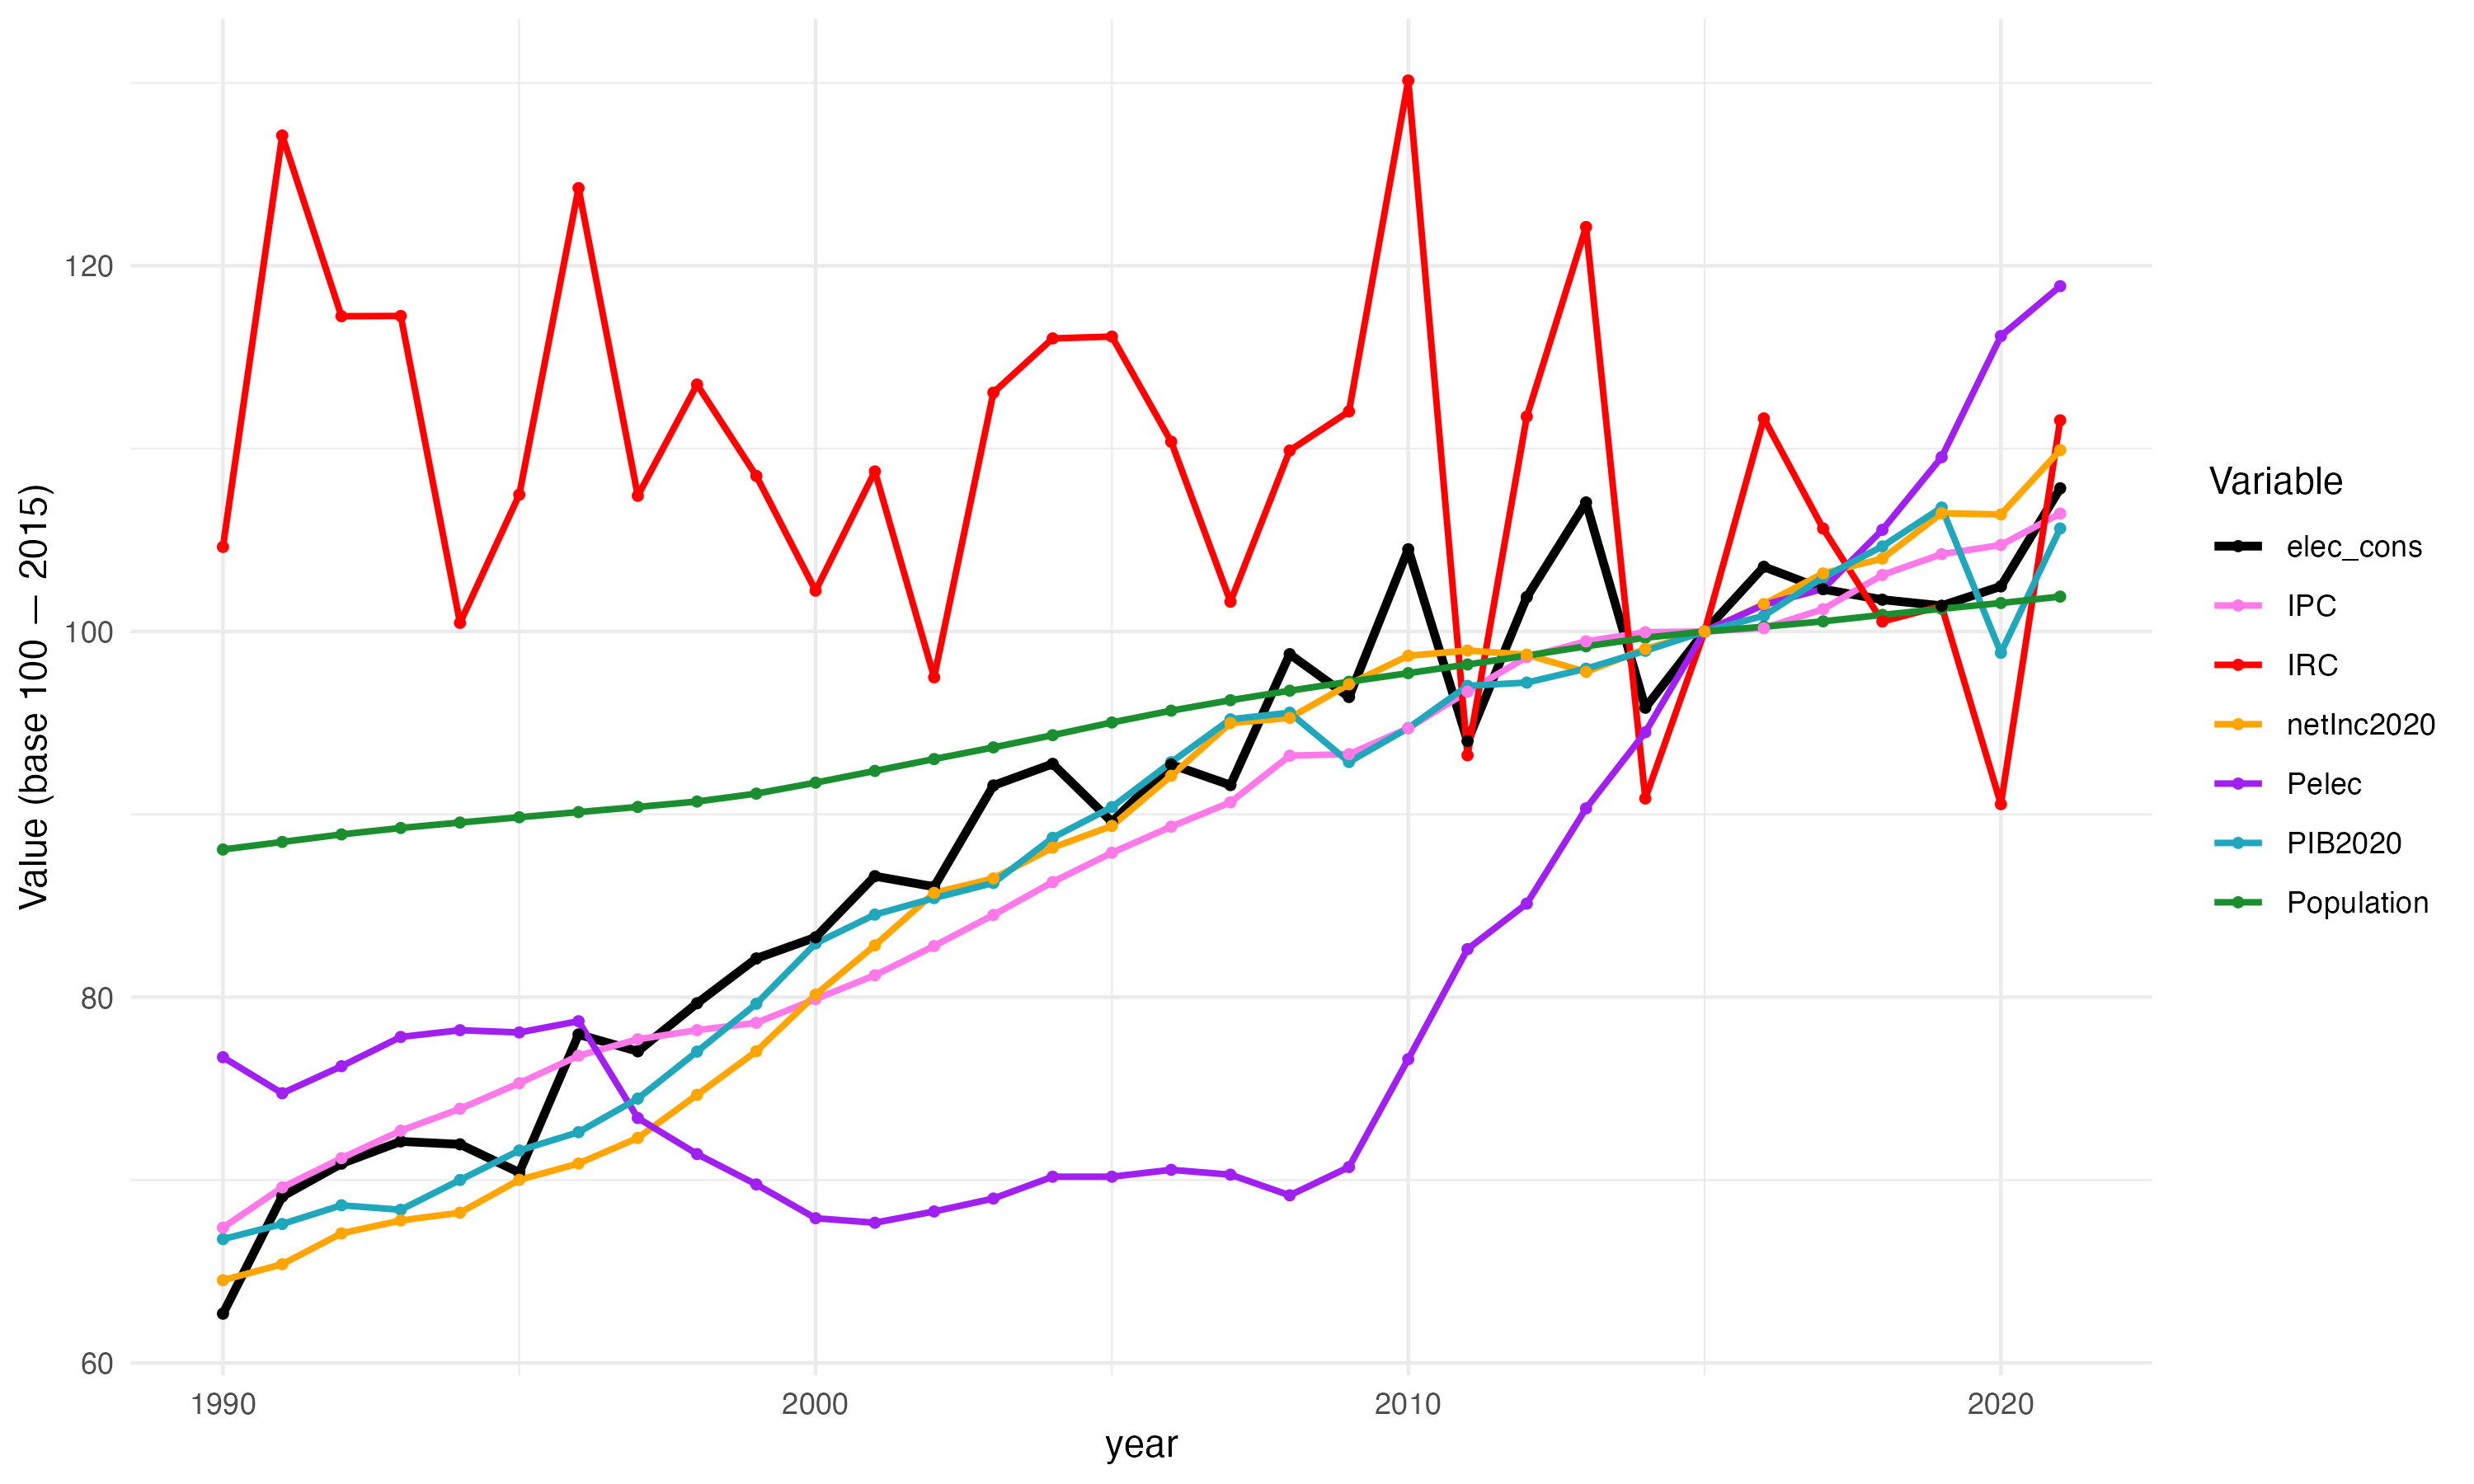
\includegraphics[width=0.5\textwidth]{Images/data_base100_2015.jpeg}
      \caption{Time variation in our data, expressed in base 100 (2015). In black the electricty consumption. In light blue and orange, respectively the GDP and the net disposable income, in euros 2020. In pink, the inflation through CPI, in green the population size. In red the climate index, and eventually in purple the electricity price.}
    \label{fig:var}
  \end{figure}

From figure \ref{fig:var}, we realize how close the GDP and the net disposable income are, only clearly diverging in trend in 2008 and 2020, which we can identify as the 2008 financial crisis and the Covid-19 crisis. Let us note that from 2008, the growth rate of electricity price becomes greater than inflation.

It seems of great matter to take into account the climate variable into our regression model, considering how electricity consumption peaks in cold winters. Eventually, we guess a correlation between the trend decline in the growth rate of electricity consumption and the burst in the price of electricity since 2009. It is likely that this sharp increase is a consequence of the 2008 energy crisis (which might be explained as the interaction of a strong positive demand shock and the ongoing financial crisis, maybe combined with the conventional oil peak that occurred around 2005-2008 \cite{delannoy2021peak}). Some market effect could also be considered, as competitive electricity markets are at play in the UE since 2007, and the treaty of Lisbon entered into force in 2009.

\begin{figure}[h]
    \centering
    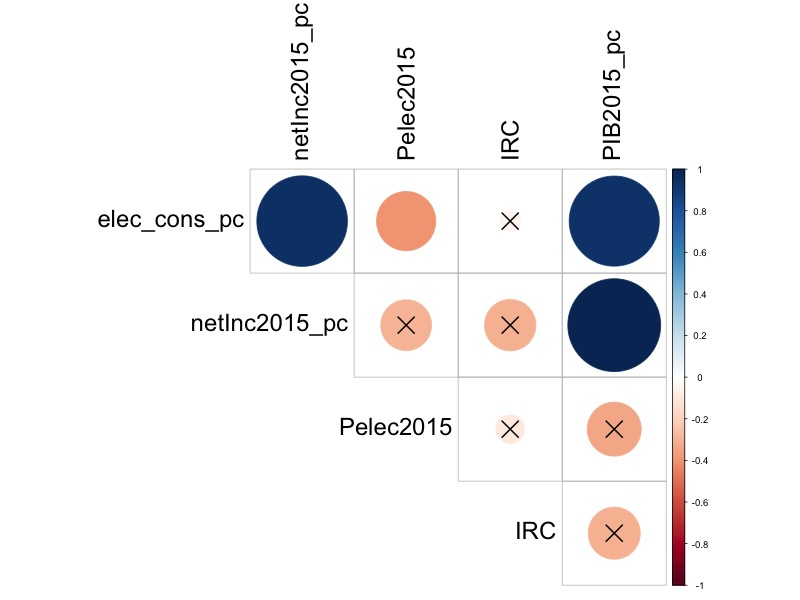
\includegraphics[width=0.5\textwidth, trim={0 0 0 5pt}, clip]{Images/correlation_matrix.jpeg}
        \caption{A correlation matrix of some data of interest. A cross indicate a p-value higher than 0.05 (no significant correlation).}
    \label{corr_mat}
  \end{figure}

The figure \ref{corr_mat} informs us of the correlation between some variable of interests, namely the electricty consumption per capita (\texttt{elec\_conc\_pc}), the net income per capita (\texttt{netInc2015\_pc}) and GDP per capita (\texttt{PIB2015\_pc}), the electricity price (\texttt{Pelec2015}) and the climate index (\texttt{IRC}). It reinforces our idea that the electricity consumption is negatively correlated with its price, and on the contrary that net disposable income and GDP are strongly correlated and might be used interchangeably.

Given our dataset, we'll tend to build simple, economically interpretable models rather than aiming for the best predictions with more complex models: we'll prioritize the comprehensibility of mechanisms over their precision.

\section{OLS Regression: a kind reminder}
For $n$ observations and $k$ variables, we use the following linear regression model:
\begin{align*}
    \boldsymbol{Y} & = \boldsymbol{X} \boldsymbol{\beta} + \boldsymbol{\varepsilon} \\
    \begin{bmatrix} 
        y_1 \\ y_2 \\ \vdots \\ y_n 
        \end{bmatrix} & = \begin{bmatrix}
        x_{11} & x_{12} & \cdots & x_{1k} \\ 
        x_{21} & x_{22} & \cdots & x_{2k} \\ 
        \vdots & \vdots & \ddots & \vdots \\ 
        x_{n1} & x_{n2} & \cdots & x_{nk} 
        \end{bmatrix} \begin{bmatrix}
        \beta_1 \\ \beta_2 \\ \vdots \\ \beta_k 
        \end{bmatrix} + \begin{bmatrix} 
        \varepsilon_1 \\ \varepsilon_2 \\ \vdots \\ \varepsilon_n \end{bmatrix}
\end{align*}

Ordinary Least Square (OLS) method is used to estimate the coefficients $\boldsymbol{\beta}$. It holds over the following hypothesis:
\begin{enumerate}
    \item More observations than explanatory variables.
    \item Absence of multicollinearity (mandatory assumption).
    \item Explanatory variables rely on data and the error term is random.
    \item The expected value of the error term is zero.
    \item Errors are not autocorrelated.
    \item Errors are homoscedastic.
    \item The error terms follow a normal distribution (for good properties).
\end{enumerate}

If the hypotheses 4, 5 and 6 are verified, the error term is a white noise (WN). 

The $R^2$ coefficient is used to evaluate the goodness of fit of the model. It measures the proportion of the variance in the dependent variable that is predictable from the independent variables. The adjusted $R^2$ is used to compare the goodness of fit of models with different numbers of variables.

Confidence interval for $\beta_j \in \{\beta_1, \beta_2, \ldots, \beta_k\}$ is given by a Student's t-distribution with $n - k - 1$ degrees of freedom.

\section{First models}
The regression equation \eqref{eq:reg} is a model of electricity consumption seeking to explain the logarithm of per capita electricity consumption by the logarithm of income per capita in constant currency and the logarithm of the price of electricity in constant currency. 

\begin{equation} \label{eq:reg}
\ln{\frac{c_{elec_i}}{pop_i}} = \alpha + \beta_1 \ln{\frac{{netInc_i}}{pop_i}} + \beta_2 \ln{\frac{price_{elec_i}}{IPC_i}} + \beta_3 IRC_i + \varepsilon_i
\end{equation}

From an economic point of view, the consumption of a good could be explained by an income effect and a price effect, to which other effects may be added if necessary. Here, we add the Climate Rigor Index (\textit{Indice de Rigueur Climatique}, IRC) to control for climate variation (\textit{e.g.} a colder winter increases electricity consumption).

$\beta_1$ and $\beta_2$ represent respectively the income elasticity and the price elasticity of electricity consumption, \textit{i.e.} the percentage change in electricity consumption in relation, respectively, to a percentage change in income and the percentage change in prices. 

The table \ref{regression_full_pc} could have shown predictable results, as the income elasticity is positive (the bigger the income the bigger the consumption) and the price elasticity is negative (the bigger the price the smaller the consumption) and low (because electricity is a necessity, the demand might be inelastic to prices). However, the latter is not well captured by the model: the price coefficient is not significant. We thus decide to add an interaction term between income and price to the model, as in equation \eqref{eq:good} (setting $y_i = \ln{\left(\frac{c_{elec_i}}{pop_i}\right)}$). 
\begin{align} \label{eq:good}
    &y_i = \alpha + \beta_1 \ln{\left(\frac{{netInc_i}}{pop_i}\right)} + \beta_2 \ln{\left(\frac{price_{elec_i}}{IPC_i}\right)} \notag \\
    &+ \beta_3 IRC_i + \beta_4 \ln{\left(\frac{{netInc_i}}{pop_i}\right)} \times \ln{\left(\frac{price_{elec_i}}{IPC_i}\right)} + \varepsilon_i
\end{align}
Let us see if the OLS assumptions hold. 

\subsection{Multicollinerarity}
The Variance Inflation Factor (VIF) of all variables but IRF was over $2000$, indicating huge multicollinearity. Because of the few variables and the small sample size we have, variable selection and regularization methods like LASSO or Elastic Net would not make any sense. In order to keep the interaction, we apply mean-centering to our variables of interests.
\begin{equation} \label{eq:mean-cent-operator}
    \begin{cases}
    \text{ln-Inc-pc} = \ln{\left(\frac{{netInc_i}}{pop_i}\right)} = X_1 & \Rightarrow {X}_1^{(MC)} = X_1 - \bar{X}_1\\
    \text{ln-price2015} = \ln{\left(\frac{price_{elec_i}}{IPC_i}\right)} = X_2 & \Rightarrow {X}_2^{(MC)} = X_2 - \bar{X}_2\\
    \end{cases}
\end{equation}

The regression therefore becomes: 
\begin{align} \label{eq:OLS-mean-cent}
    & y_i = \alpha + \beta_1 \left(\text{ln-Inc-pc}_i^{(MC)}\right) + \beta_2 \left(\text{ln-price2015}_i^{(MC)}\right) \notag \\
    & + \beta_3 IRC_i + \beta_4 \left(\text{ln-Inc-pc}_i^{(MC)} \times \text{ln-price2015}_i^{(MC)}\right) + \varepsilon_i
\end{align}
Using model \eqref{eq:OLS-mean-cent}, we don't face multicollinearity anymore: our VIF values for all variables stands between $1$ and $3$. The following tests are performed on this model.

\subsection{Normality of residuals}
It is known that the Kolmogorov-Smirnov test is less powerful for testing normality than the Shapiro-Wilk test or Anderson-Darling test. Because the Shapiro-Wilk does not work well with many identical values and the Jarque-Bera test is not efficient for small samples, we choose the Anderson-Darling test to see whether the error terms follow a normal distribution. The test provides a p-value of $0.2989$, so we do not reject the null-hypothesis that the residuals are normally distributed. Also, we performed a one sample t-test on the residuals to control for the null hypothesis that the mean of the residuals is zero, which is true.

\subsection{Homoscedasticity}
The White test can detect a wide range of forms of heteroskedasticity, but tends to falsely detect heteroscedasticity in small samples. The {Breusch-Pagan} test is designed to detect only linear forms of heteroskedasticity, and even though the Goldfeld–Quandt test is not very robust to specification errors, it performs better for small samples. Both Breusch-Pagan and Goldfeld–Quandt tests give a p-value over $0.7$, so we can admit that the residuals are homoscedastic.

\subsection{Autocorrelation}
Three tests can be used: the Durbin-Watson test is valid for nonstochastic regressors and allows to test the possibility of a first-order autoregressive model (e.g. AR(1)) for the regression errors. The Ljung-Box test, which requires the assumption of strict exogeneity, controls for higher order autocorrelation. 
The Breusch–Godfrey test is statistically more powerful than Durbin's h statistic and more general than the {Ljung-Box} test. It checks for serial correlation and requires the assumptions of stronger forms of predeterminedness and conditional homoscedasticity.

Performing the tests (see table \ref{autocorrelation_tests}) reveals that the model does not suffer from autocorrelation, the residuals are independent, even we looking at multiple lags.
\begin{table}[h]
    \centering
    \caption{Autocorrelation Test Results}
    \label{autocorrelation_tests}
    \begin{tabular}{lccc}
    \\[-1.8ex]\hline 
    \hline \\[-1.8ex] 
    Test & Statistic & DF & p-value \\
    \hline
    Durbin-Watson & 1.7639  & NA & 0.1066 \\
    Ljung-Box (lag=10) & 11.8304  & 10 & 0.2966 \\
    Breusch-Godfrey & 0.1482  & 1 & 0.7003 \\
    \hline
    \end{tabular}
\end{table}

\subsection{Results}
The model \eqref{eq:OLS-mean-cent} passed all the tests: it is well specified and can be interpreted. The table \ref{regression_good_linear} shows the results of the regression. The $R^2$ and adjusted $R^2$ are around 0.96, meaning that the model explains most of the variance in the dependent variable. The F-statistic is high with $p-value < 2.2e-16$, meaning that the model is statistically significant. 

\begin{table}[!htbp] \centering 
    \caption{Regression analysis results from model \eqref{eq:reg}.} 
    \label{regression_full_pc} 
  \begin{tabular}{@{\extracolsep{0pt}}lc} 
  \\[-1.8ex]\hline 
  \hline \\[-1.8ex] 
   & \multicolumn{1}{c}{\textit{Dependent variable:}} \\ 
  \cline{2-2} 
  \\[-1.8ex] & log(elec\_cons\_pc) \\ 
  \hline \\[-1.8ex] 
   log(netInc2015\_pc) & 0.859$^{***}$ \\ 
    & (0.044) \\ 
    & \\ 
   log(Pelec2015) & $-$0.057 \\ 
    & (0.039) \\ 
    & \\ 
   IRC & 0.269$^{***}$ \\ 
    & (0.057) \\ 
    & \\ 
   Constant & $-$9.563$^{***}$ \\ 
    & (0.212) \\ 
    & \\ 
  \hline \\[-1.8ex] 
  Observations & 32 \\ 
  R$^{2}$ & 0.944 \\ 
  Adjusted R$^{2}$ & 0.938 \\ 
  Residual Std. Error & \makecell{0.026 \\ (df = 28)} \\  % Multi-line with makecell
    F Statistic & \makecell{157.060$^{***}$ \\ (df = 3; 28)} \\  % Multi-line with makecell 
  \hline 
  \hline \\[-1.8ex] 
  \textit{Note:}  & \multicolumn{1}{r}{$^{*}$p$<$0.05; $^{**}$p$<$0.01; $^{***}$p$<$0.001} \\ 
  \end{tabular} 
\end{table} 

\begin{table}[!htbp] \centering 
    \caption{Regression analysis results from model \eqref{eq:OLS-mean-cent}.} 
    \label{regression_good_linear} 
    \begin{tabular}{@{\extracolsep{0pt}}lc} 
        \\[-1.8ex]\hline 
        \hline \\[-1.8ex] 
         & \multicolumn{1}{c}{\textit{Dependent var.:}} \\ 
        \cline{2-2} 
        \\[-1.8ex] & log(elec\_cons\_pc) \\ 
        \hline \\[-1.8ex] 
         ln\_Inc\_pc\_MC & 0.720$^{***}$ \\ 
          & (0.055) \\ 
          & \\ 
         ln\_price2015\_MC & $-$0.104$^{**}$ \\ 
          & (0.036) \\ 
          & \\ 
         IRC & 0.293$^{***}$ \\ 
          & (0.049) \\ 
          & \\ 
         ln\_Inc\_pc\_MC:ln\_price2015\_MC & 1.348$^{**}$ \\ 
          & (0.387) \\ 
          & \\ 
         Constant & $-$13.295$^{***}$ \\ 
          & (0.049) \\ 
          & \\ 
        \hline \\[-1.8ex] 
        Observations & 32 \\ 
        R$^{2}$ & 0.961 \\ 
        Adjusted R$^{2}$ & 0.956 \\ 
        Residual Std. Error & \makecell{0.022 \\ (df = 27)} \\ 
        F Statistic & \makecell{167.504$^{***}$ \\ (df = 4; 27)} \\ 
        \hline 
        \hline \\[-1.8ex] 
        \textit{Note:} $^{*}$p$<$0.05; $^{**}$p$<$0.01; $^{***}$p$<$0.001  & \multicolumn{1}{r}{} \\ 
    \end{tabular} 
\end{table} 
        

In the model $y_i = \alpha + \beta_1 X_{1_i} + \beta_2 X_{2_i} + \beta_3 X_{3_i} + \beta_4  X_{1_i} X_{2_i} + \varepsilon_i$, the elasticity of $X_j$ on $y$ is given by $\frac{\partial y}{\partial X_j}$. Therefore, the new net income per capita and price elasticities of electricity consumption are defined as: 
\begin{equation} \label{eq:elast}
    \begin{cases}
    \text{Income elast.:} & \beta_{Inc} = \beta_1 + \beta_4 \text{ln-price2015}^{(MC)}\\
    \text{Price elast.:} & \beta_{price} =\beta_2 + \beta_4 \text{ln-Inc-pc}^{(MC)} \\    
    \end{cases}
\end{equation}

Because of the mean-centering, $\beta_1$ and $\beta_2$ capture the baseline effect of a variable at its sample mean while $\beta_4$ represents how the effect of price depends on income in relation to the average income per capita level.

The new elasticites expression given equation \eqref{eq:elast} are precious to understand the regression coefficients given table \ref{regression_good_linear}, as it can be shown that for any observation $i$, $\beta_{Inc} > \beta_1 = 0.720$ and $\beta_{price} < \beta_2 = -0.104$ (because $\forall i, \text{ln-price2015}^{(MC)}_i > 0$ and $\text{ln-Inc-pc}^{(MC)}_i < 0$). 

Thus, classic microeconometric results are found as there is a negative price elasticity and a positive income elasticity of electricity consumption. The more expensive electricity is, the less people will consume it, and the richer they are, the more they will consume. We should nonetheless highlight the fact that the upper bound of $\beta_{price}$, $\beta_2$, is close to an inelasticity threshold: because electricity is a necessary good, the price effect is lower than the income effect, due to the households' non-compressible electricity consumption. $\beta_3$ value also leads to an obvious result: the colder a winter is, the more electricity is consumed.

The interaction term is positive, meaning that the price elasticity of electricity consumption increases with income. If income increases, the price effect becomes less negative: this could be explained by the fact that after a certain level of income, households are less sensitive to price changes. On the other way around, if electricity prices rise, income has a stronger positive effect on consumption.

\section{Structural break}
\subsection{Eliciting the break date}
We previously mentioned how 2008 seemed to be a turning point in the electricity price trend and how it could have affected the electricity consumption trend. Let us use statistical techniques to detect whether or not this break matters. 

Bai and Perron (1998, 2003) provided a theoretical framework and computational algorithms to estimate and test for multiple structural changes at unknown dates in linear regression models, where the regressors are non-trending or regime-wise stationary \cite{bai1998estimating, bai2003computation}. 

The Bai-Perron multiple break test \cite{bai1998estimating} identifies $m$ breakpoints as $t_1^, t_2^, \dots, t_m^*$ by minimizing the sum of squared residuals (SSR) across different segments. 

$$\sum_{j=1}^{m+1} SSR(y_{t_{j-1}+1:t_j})$$

where $t_0 = 1$ and $t_{m+1} = T$. 

First, by computing the sequential $\sup F$ tests of $l$ versus $l+1$ for $l \in \{1, \dots, m\}$ with each corresponding null hypothesis of maximum number of break is $l$ and alternative hypothesis is $l+1$, we can identify the number of breakpoints. Then, knowing the number of breakpoints, we can compute a structural change model and split the dataset into separate regimes. 

Therefore, Bai-Perron Test is particularly useful as it can found multiple unkown breaks while handling potential heteroskedasticity and serial correlation.

On the contrary, the Chow test \cite{chow1960tests} is used to check whether a structural break occurs at a specific, pre-determined date, assuming OLS properties. To perform a Chow test, we need to split the sample at the known break date into two subsamples. Then, we estimate the regression separately for both subsamples and for the entire dataset (without a break). To test whether the coefficients before and after the break are significantly different, we use the following F-statistics:
$$F = \frac{(SSR_r - (SSR_1 + SSR_2)) / k}{(SSR_1 + SSR_2) / (n_1 + n_2 - 2k)}$$

where $SSR_r$ is Sum of squared residuals for the full model, $SSR_1, SSR_2$ the one for the "before" and "after" models, $k$ the number of parameters in the model and $n_1, n_2$ the number of observations in each segment. 

The Bai-Perron test indicates that there are two breaks in the data (see table \ref{tab:supF_tests}) and finds them in 1999 and 2007 (see figure \ref{fig:bai-perron-break}). To substantiate this result, we perform a step-by-step Chow test between 2006 and 2011 to determine the most likely break date. Figure \ref{fig:chow-break} also suggests a break date in 2007, which is consistent with the Bai-Perron test. It is clear that the latest break date is related with the oil peak and the financial crisis of 2008. The first break date suggested by Bai-Perron is less obvious but might be related to the 1999 storm that hit France and disrupted 8\% of the electricity grid system\footnote{See \href{https://www.osti.gov/etdeweb/servlets/purl/20222814}{RTE}.}. On the latter, we will focus on 2007 as the year in which structural change occurred.

\begin{table}[!htbp] 
    \centering
    \caption{Bai-Perron test for structural breaks, looking for the optimal number of breaks.} \vspace{0.1cm}
    \label{tab:supF_tests}
    \textit{supF(l+1|l) tests using global optimizers under the null.}
    \begin{tabular}{lccc}
        % \\[-1.8ex]\hline 
        % \hline \\[-1.8ex] 
        \\[-1.8ex] \toprule
        & \textbf{supF(1|0)} & \textbf{supF(2|1)} & \textbf{supF(3|2)} \\
        \midrule
        Seq supF & 34.725 & 79.941 & 12.626 \\
        \midrule
        10\% CV  & 11.590 & 13.430 & 14.430 \\
        5\% CV   & 13.470 & 15.250 & 16.360 \\
        2.5\% CV & 15.280 & 17.080 & 18.100 \\
        1\% CV   & 17.600 & 19.350 & 20.020 \\
        \bottomrule
    \end{tabular}
\end{table}

\begin{figure}[h]
    \centering
      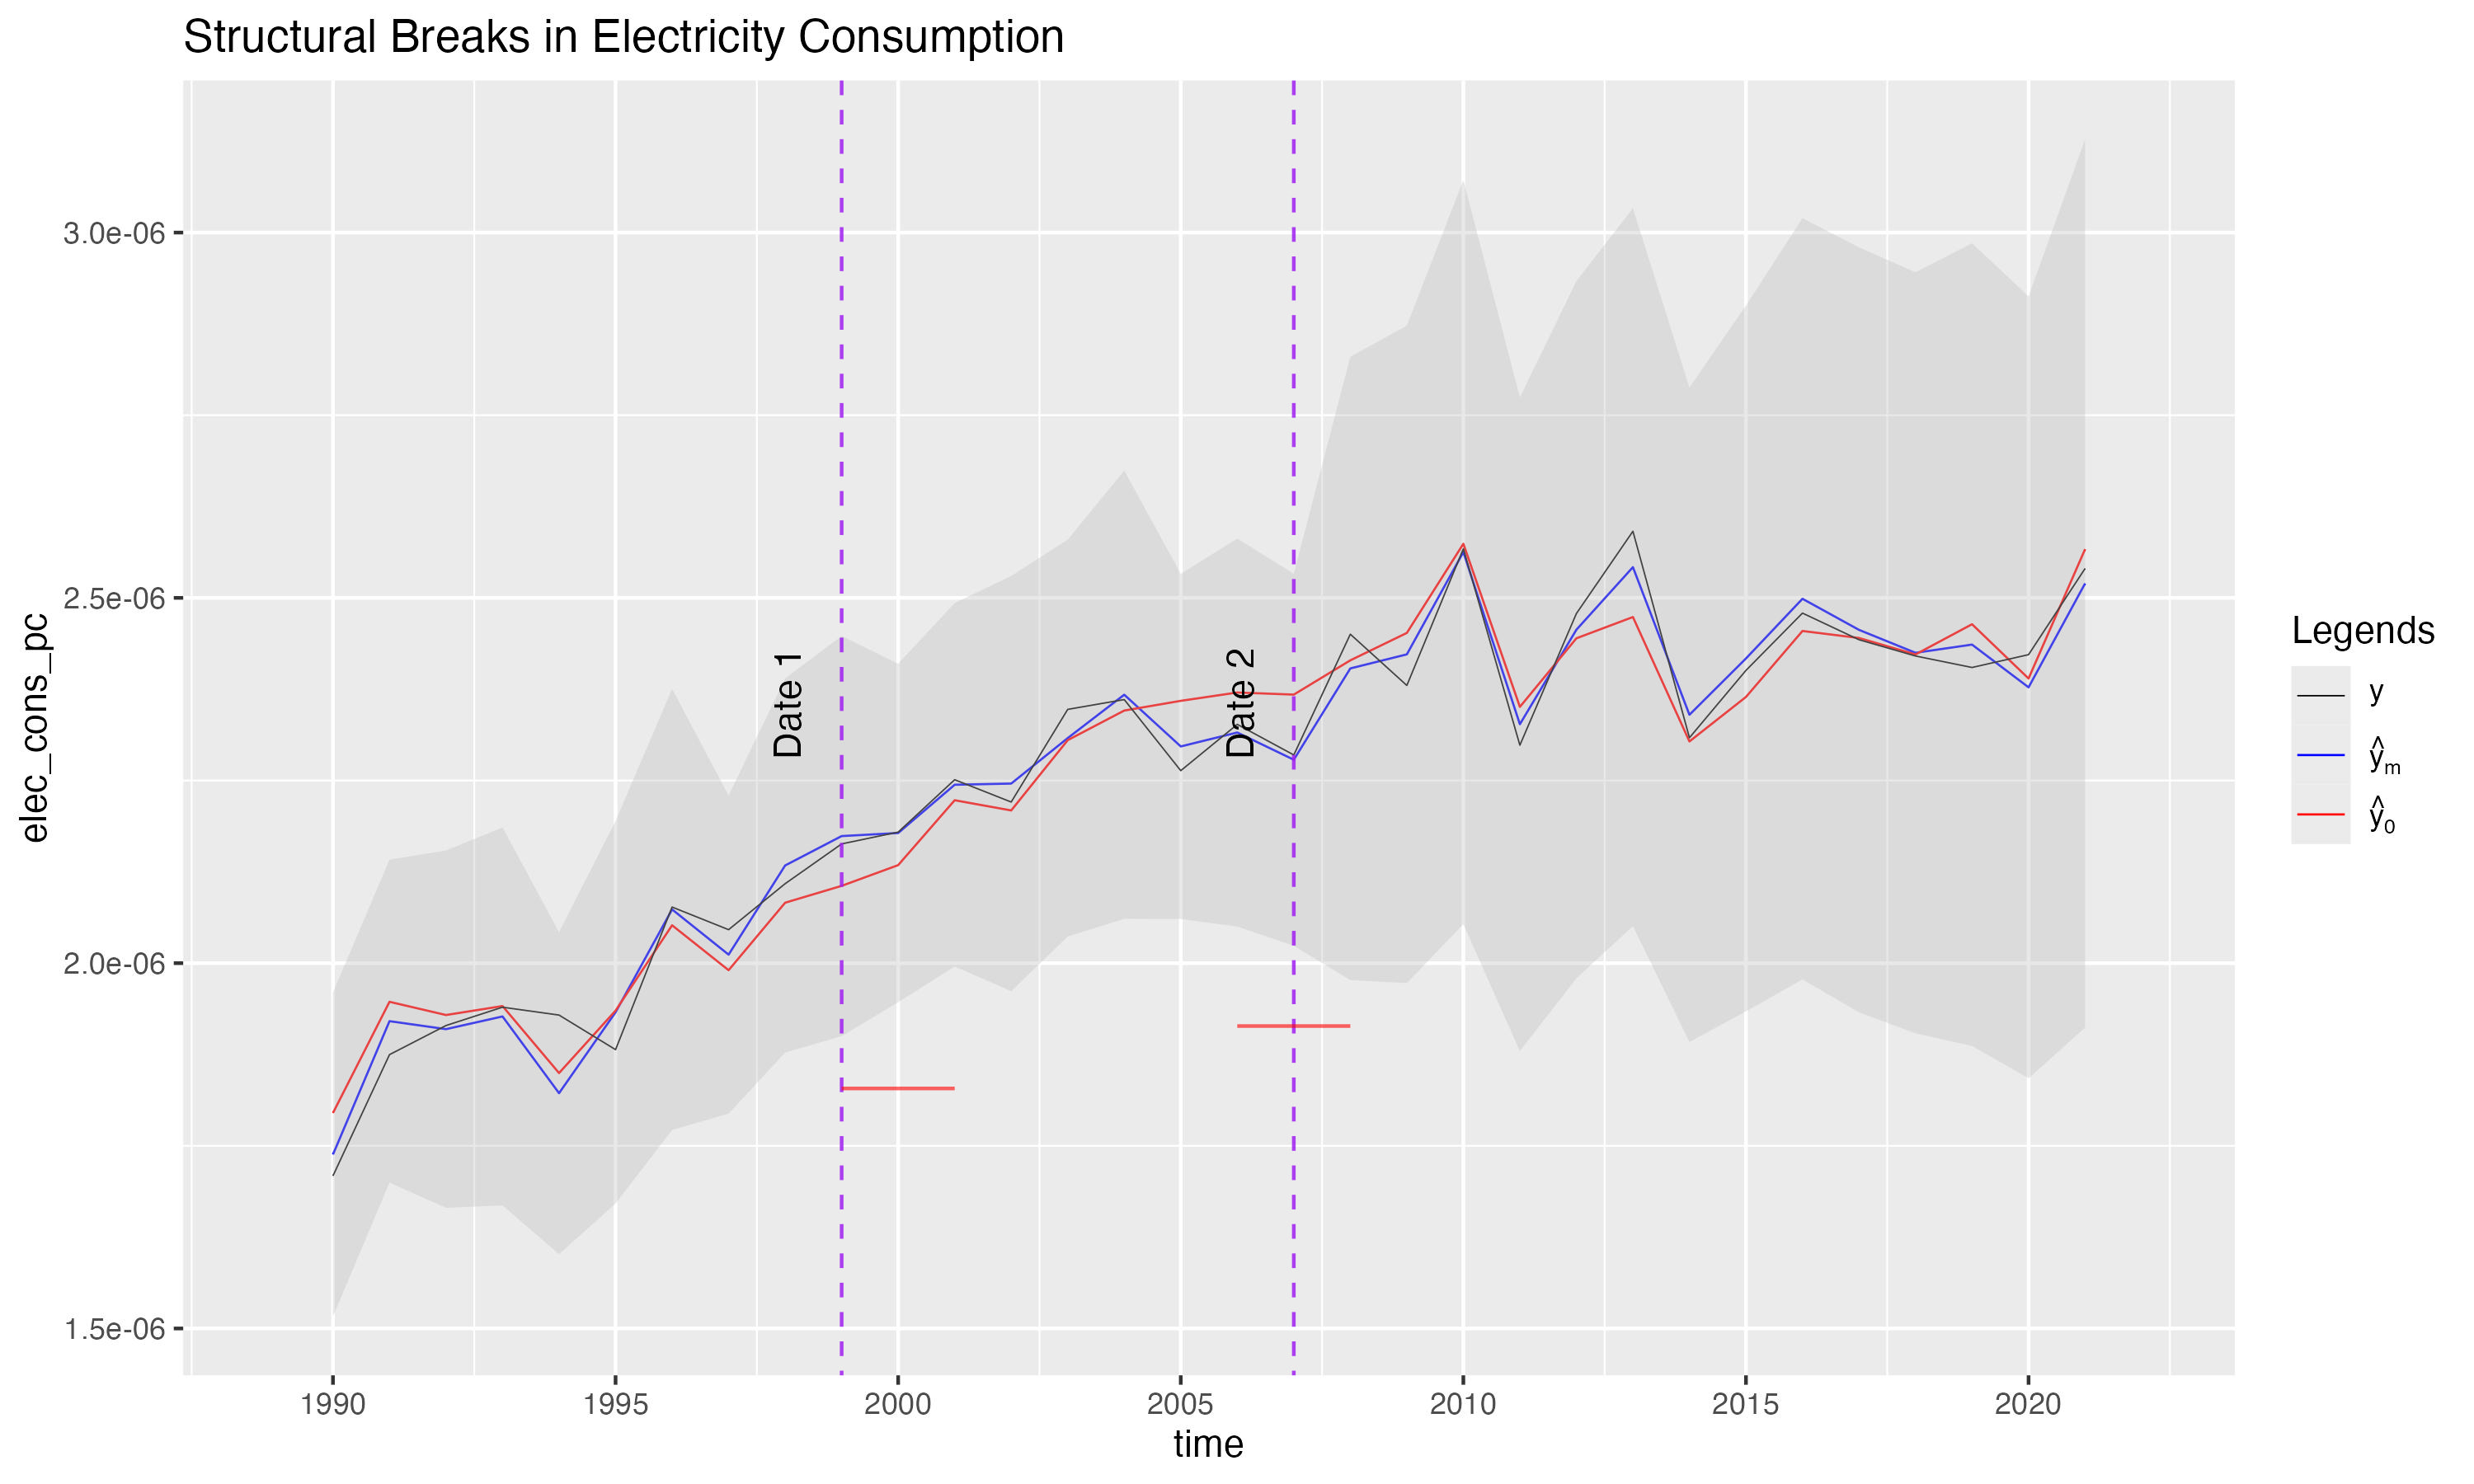
\includegraphics[width=0.5\textwidth]{Images/structural_breaks.jpeg}
      \caption{Bai-Perron test for structural breaks, looking for two breaks in the mean-centered log of electricity price and net disposable income in constant currency.}
    \label{fig:bai-perron-break}
  \end{figure}

\begin{figure}[h]
    \centering
      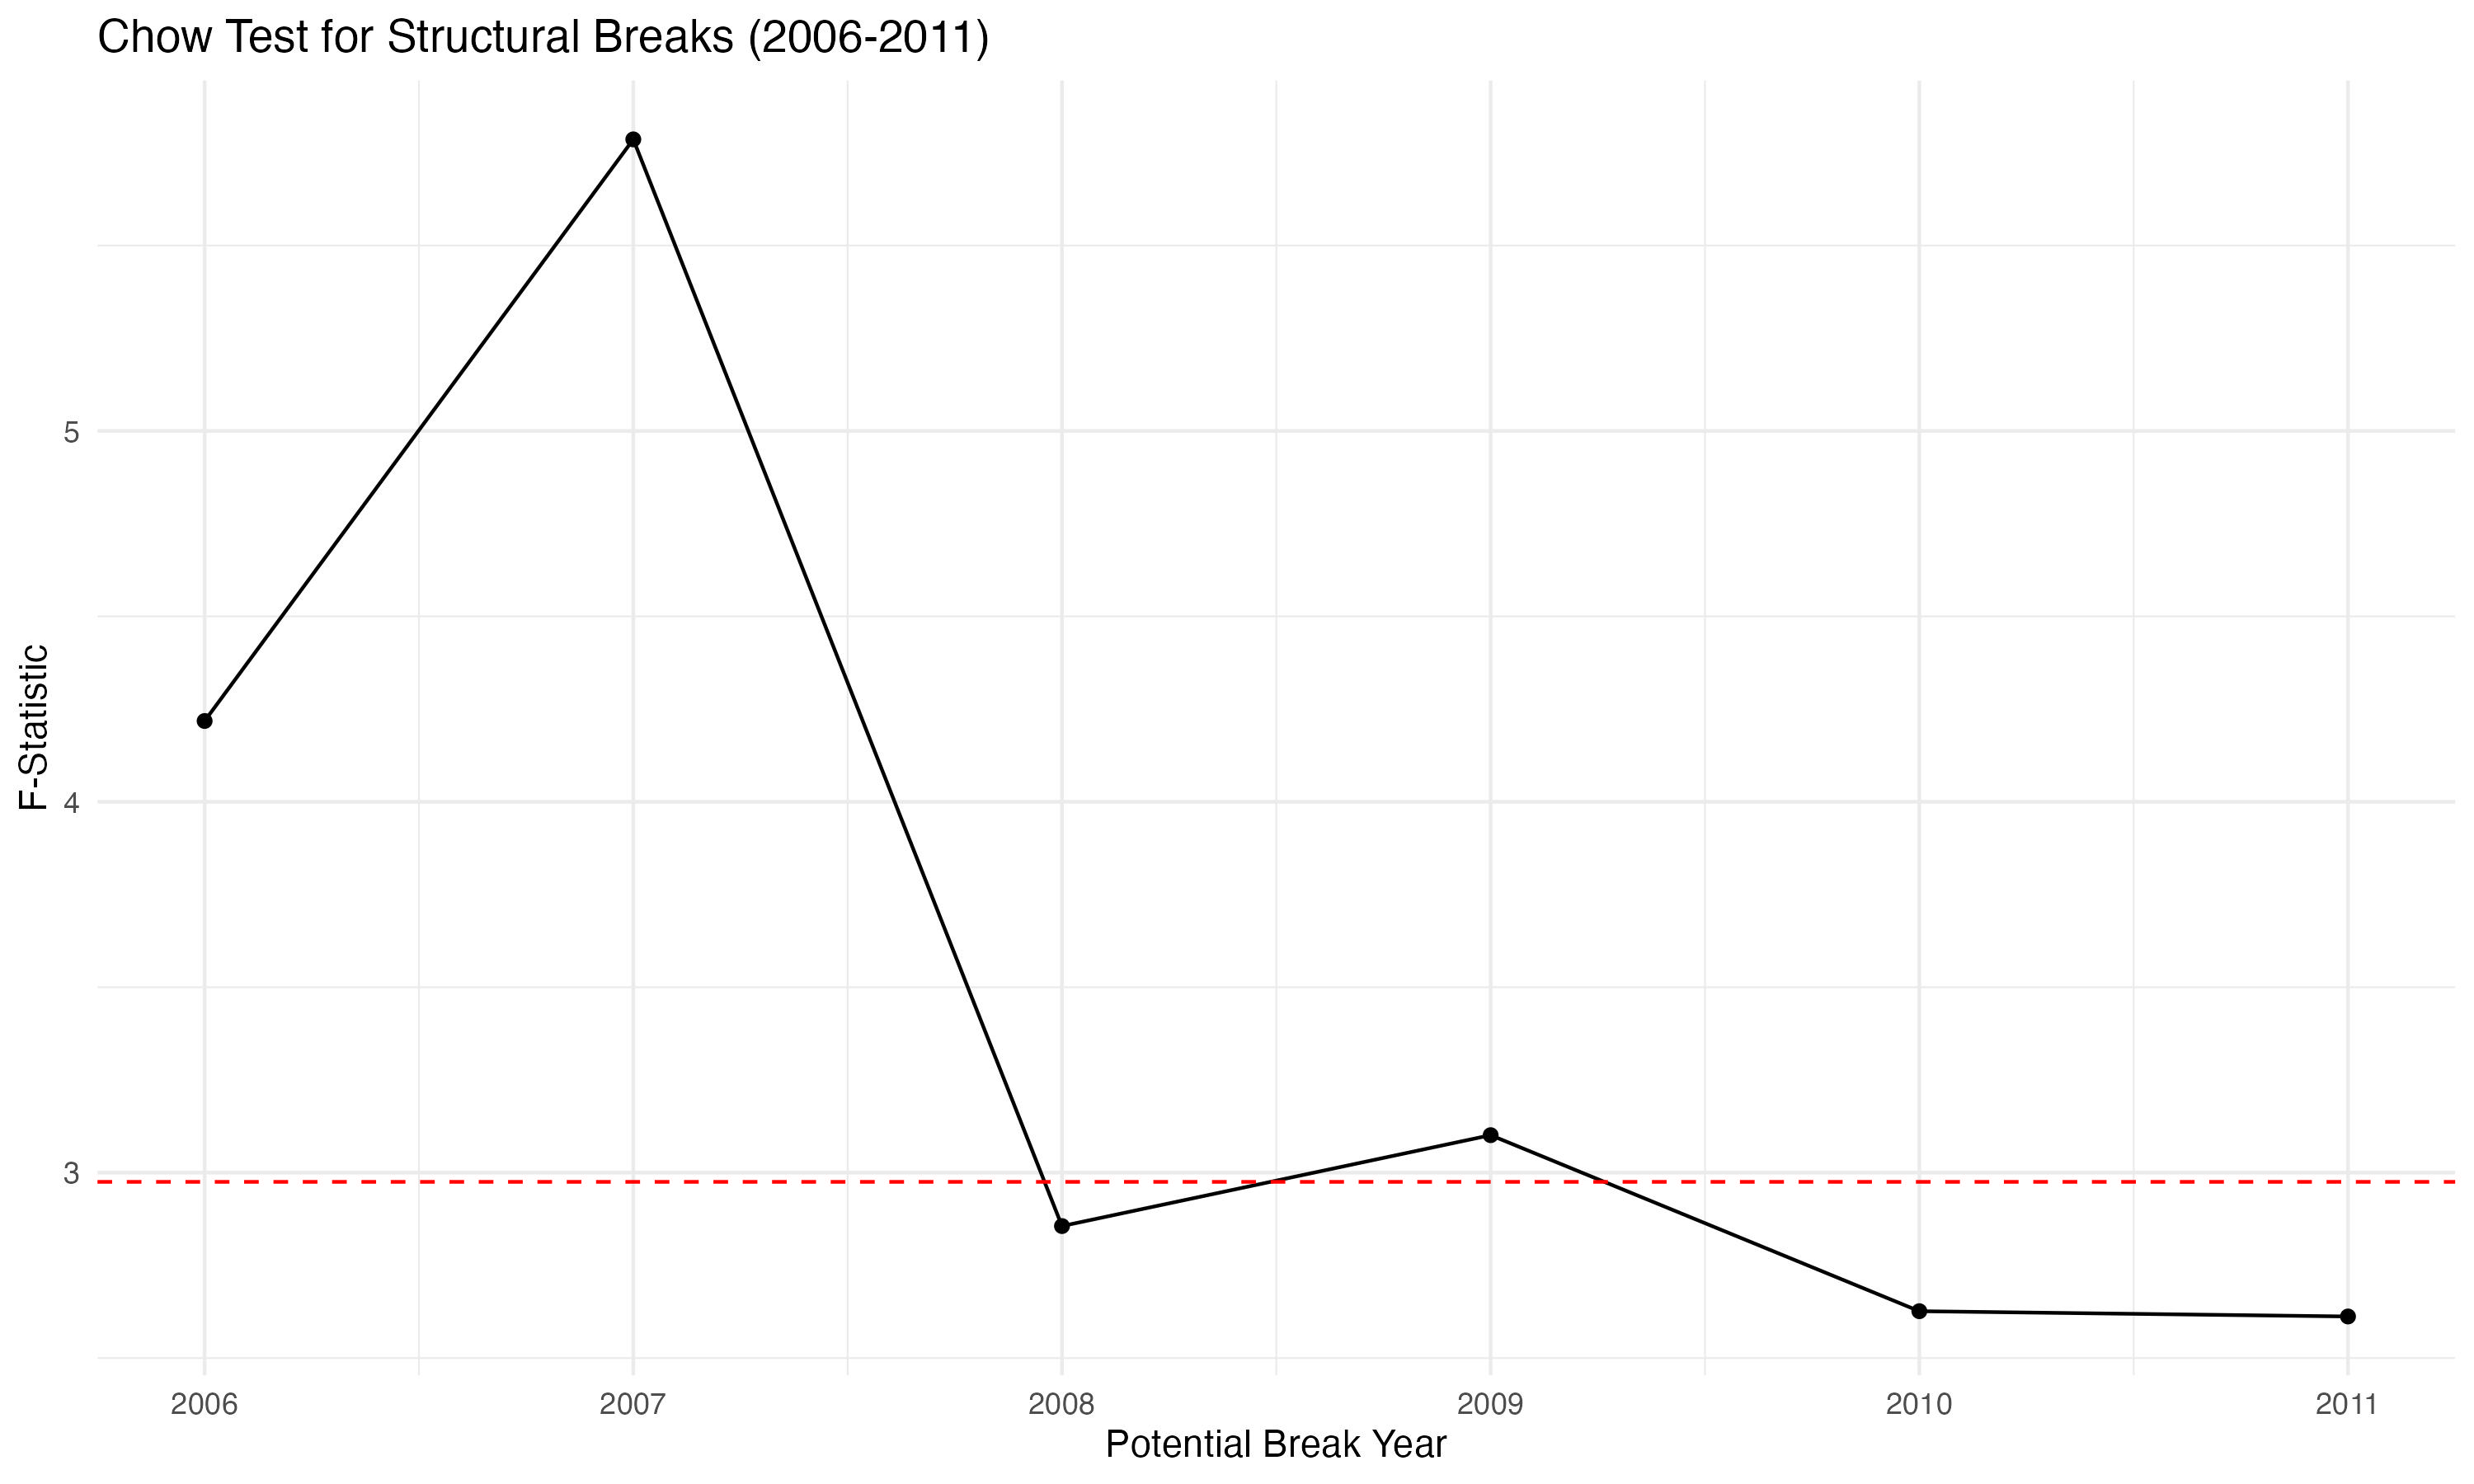
\includegraphics[width=0.5\textwidth]{Images/chow_test_results.jpeg}
      \caption{Step-by-step Chow test results on the model \ref{eq:OLS-mean-cent} between 2006 and 2011. Each point above the dashed red line indicates a significant break. We retain as the break date the one with the highest F-statistic.}
    \label{fig:chow-break}
\end{figure}

One should note that the COVID-19 crisis in 2020 is not detected, because of the lack of data coming after this date (our dataset ends in 2021). However, using net disposable income instead of GDP also seems to avoid the effect of the COVID-19 crisis, as no break appears on figure \ref{fig:var}. Furthermore, there are no evidence that electricity prices have been affected by the COVID-19 crisis, the recent spike in prices being more likely due to the war in Ukraine and the economic recovery.

\subsection{Taking into account the structural break}
Perfoming a regression on the last subset of date ($> 2007$) using the model \eqref{eq:OLS-mean-cent} elicits strong multicollinearity between the price and the interaction term. Because our independent variables are already mean-centered and the sample size is small and we have a low degree of freedom, regularization methods (\textit{e.g.} Ridge) would not be efficient.

To explore how the break affects the model, we introduce a dummy variable that takes the value $1$ after the break date and $0$ before. The model \eqref{eq:break} is then estimated using OLS. The results are shown in table \ref{regression_break}: the dummy is significant, \textit{i.e.} the structural break has an impact on the electricity consumption. 

\begin{align} \label{eq:break}
    & y_i = \alpha + \beta_1 \left(\text{ln-Inc-pc}_i^{(MC)}\right) + \beta_2 \left(\text{ln-price2015}_i^{(MC)}\right) \notag \\
    & + \beta_3 IRC_i + \beta_4 \left(\text{ln-Inc-pc}_i^{(MC)} \times \text{ln-price2015}_i^{(MC)}\right) \notag \\
    & + \beta_5 \text{Break}_i + \varepsilon_i \notag \\
     \notag \\
    & \text{with} \quad \text{Break}_i = \begin{cases}
    1 & \text{if } t_i > 2007 \\
    0 & \text{otherwise}
    \end{cases} 
\end{align}
\begin{table}[!htbp] \centering 
    \caption{Regression analysis results from model \eqref{eq:break}.} 
    \label{regression_break} 
  \begin{tabular}{@{\extracolsep{0pt}}lc} 
  \\[-1.8ex]\hline 
  \hline \\[-1.8ex] 
   & \multicolumn{1}{c}{\textit{Dependent var.:}} \\ 
  \cline{2-2} 
  \\[-1.8ex] & log(elec\_cons\_pc) \\ 
  \hline \\[-1.8ex] 
   ln\_Inc\_pc\_MC & 0.474$^{***}$ \\ 
    & (0.095) \\ 
    & \\ 
   ln\_price2015\_MC & $-$0.194$^{***}$ \\ 
    & (0.044) \\ 
    & \\ 
   IRC & 0.279$^{***}$ \\ 
    & (0.043) \\ 
    & \\ 
   break\_dummy & 0.047$^{**}$ \\ 
    & (0.016) \\ 
    & \\ 
   ln\_Inc\_pc\_MC:ln\_price2015\_MC & 1.969$^{***}$ \\ 
    & (0.398) \\ 
    & \\ 
   Constant & $-$13.299$^{***}$ \\ 
    & (0.043) \\ 
    & \\ 
  \hline \\[-1.8ex] 
  Observations & 32 \\ 
  R$^{2}$ & 0.971 \\ 
  Adjusted R$^{2}$ & 0.966 \\ 
  Residual Std. Error & \makecell{0.020 \\ (df = 26)} \\ 
  F Statistic & \makecell{175.497$^{***}$ \\ (df = 5; 26)} \\ 
  \hline 
  \hline \\[-1.8ex] 
  \textit{Note:} $^{*}$p$<$0.05; $^{**}$p$<$0.01; $^{***}$p$<$0.001  & \multicolumn{1}{r}{} \\ 
  \end{tabular} 
  \end{table} 
  
Knowing the existence of a structural break, we are looking for two models, pre-2007 and post-2007, that can elicit the reason of the change in eletricity consumption (prices, income, climate, crisis, etc.). Because using model \eqref{eq:OLS-mean-cent} on the two subsets reveals high multicollinearity, we explore what would be the best variables to include in the model with the help of the Bayesian Information Criterion (BIC) — a criterion that values the goodness of fit of a model while penalizing the number of parameters, maintaining the model's simplicity.

Equations \eqref{eq:before-after} show the two models we retained, with $\text{Crisis}_i$ being a dummy variable for the French 1999 storm, the financial crisis and the COVID-19 crisis (${Crisis}_i = 1$ for $i~=~\{1999, 2008, 2020\}, 0$~otherwise). The results are displayed in tables \ref{regression_before} and \ref{regression_after}, with the OLS assumptions (no multicollinearity and the error terms are $\varepsilon_i \sim WN(0, \sigma^2)$, {with} $\varepsilon_i \overset{iid}{\sim} \mathcal{N}(0, \sigma^2)$) being verified.
\begin{align} \label{eq:before-after}
    \begin{cases}
        \forall i \leq 2007 & y_i = \alpha + \beta_1 \left(\text{ln-Inc-pc}_i^{(MC)}\right) + \beta_3 IRC_i + \\ & \beta_4 \left(\text{ln-Inc-pc}_i^{(MC)} \times \text{ln-price2015}_i^{(MC)}\right) + \varepsilon_i \\
        \\
        \forall i > 2007 & y_i = \alpha + \beta_2 \left(\text{ln-price2015}_i^{(MC)}\right) + \beta_3 IRC_i + \\ & \beta_5 \text{Crisis}_i + \varepsilon_i
    \end{cases} 
\end{align}
The two tables highlight a clear change in regimes, the model before the break being more influenced by an income effect (the price elasticity derived from equation \eqref{eq:elast} is slightly negative and denote an inelastic demand) while the model after the break is more influenced by the climate fluctuations. An unusual result is the positive sign of $\beta_2$ in the second model. It interestingly raises the question of reverse causality, as high consumption could drive prices up, for instance in cases of supply constraints (\textit{e.g.} in 2012 or in 2017\footnote{see \href{http://publications.elia.be/upload/UG_upload/5SQMH9Z4FF.pdf}{RTE} and \href{https://www.nucnet.org/news/as-france-faces-winter-supply-constraints-iea-says-renewables-cannot-replace-nuclear}{IEA}.}), whereas there is an increasing number of electronic devices and more heating during winter. Also, during a crisis, subsidies can be distributed to face high electricity costs, which might reduce households' sensitivity to price changes such that an increase in price does not lead to a decrease in demand.

\begin{table}[!htbp] \centering 
    \caption{Regression analysis results from model \eqref{eq:before-after}, before the structural break.} 
    \label{regression_before} 
  \begin{tabular}{@{\extracolsep{0pt}}lc} 
  \\[-1.8ex]\hline 
  \hline \\[-1.8ex] 
   & \multicolumn{1}{c}{\textit{Dependent var:}} \\ 
  \cline{2-2} 
  \\[-1.8ex] & log(elec\_cons\_pc) \\ 
  \hline \\[-1.8ex] 
   ln\_Inc\_pc\_MC & 0.701$^{***}$ \\ 
    & (0.066) \\ 
    & \\ 
   IRC & 0.235$^{**}$ \\ 
    & (0.065) \\ 
    & \\ 
   ln\_Inc\_pc\_MC:ln\_price2015\_MC & 2.266$^{***}$ \\ 
    & (0.451) \\ 
    & \\ 
   Constant & $-$13.230$^{***}$ \\ 
    & (0.066) \\ 
    & \\ 
  \hline \\[-1.8ex] 
  Observations & 18 \\ 
  R$^{2}$ & 0.966 \\ 
  Adjusted R$^{2}$ & 0.958 \\ 
  Residual Std. Error & \makecell{0.019 \\ (df = 14)} \\ 
  F Statistic & \makecell{131.663$^{***}$ \\ (df = 3; 14)} \\ 
  \hline 
  \hline \\[-1.8ex] 
  \textit{Note:} $^{*}$p$<$0.05; $^{**}$p$<$0.01; $^{***}$p$<$0.001 & \multicolumn{1}{r}{} \\ 
  \end{tabular} 
  \end{table} 
  
  \begin{table}[!htbp] \centering 
    \caption{Regression analysis results from model \eqref{eq:before-after}, after the structural break.} 
    \label{regression_after} 
  \begin{tabular}{@{\extracolsep{0pt}}lc} 
  \\[-1.8ex]\hline 
  \hline \\[-1.8ex] 
   & \multicolumn{1}{c}{\textit{Dependent var.:}} \\ 
  \cline{2-2} 
  \\[-1.8ex] & log(elec\_cons\_pc) \\ 
  \hline \\[-1.8ex] 
   ln\_price2015\_MC & 0.141$^{***}$ \\ 
    & (0.020) \\ 
    & \\ 
   IRC & 0.378$^{***}$ \\ 
    & (0.026) \\ 
    & \\ 
   crisis\_dummy & 0.029$^{**}$ \\ 
    & (0.007) \\ 
    & \\ 
   Constant & $-$13.298$^{***}$ \\ 
    & (0.026) \\ 
    & \\ 
  \hline \\[-1.8ex] 
  Observations & 14 \\ 
  R$^{2}$ & 0.955 \\ 
  Adjusted R$^{2}$ & 0.942 \\ 
  Residual Std. Error & \makecell{0.008 \\(df = 10)} \\ 
  F Statistic & \makecell{71.386$^{***}$ \\ (df = 3; 10)} \\ 
  \hline 
  \hline \\[-1.8ex] 
  \textit{Note:}  & \multicolumn{1}{r}{$^{*}$p$<$0.05; $^{**}$p$<$0.01; $^{***}$p$<$0.001} \\ 
  \end{tabular} 
  \end{table} 
  
  OLS regression of models \eqref{eq:break} and \eqref{eq:before-after} are graphically displayed figure \ref{fig:regstructural}. One can get how the two submodels fit slightly better the datapoints. Still, the difference between models \eqref{eq:break} and \eqref{eq:before-after} is fairly small.

  \begin{figure}[h]
    \centering
      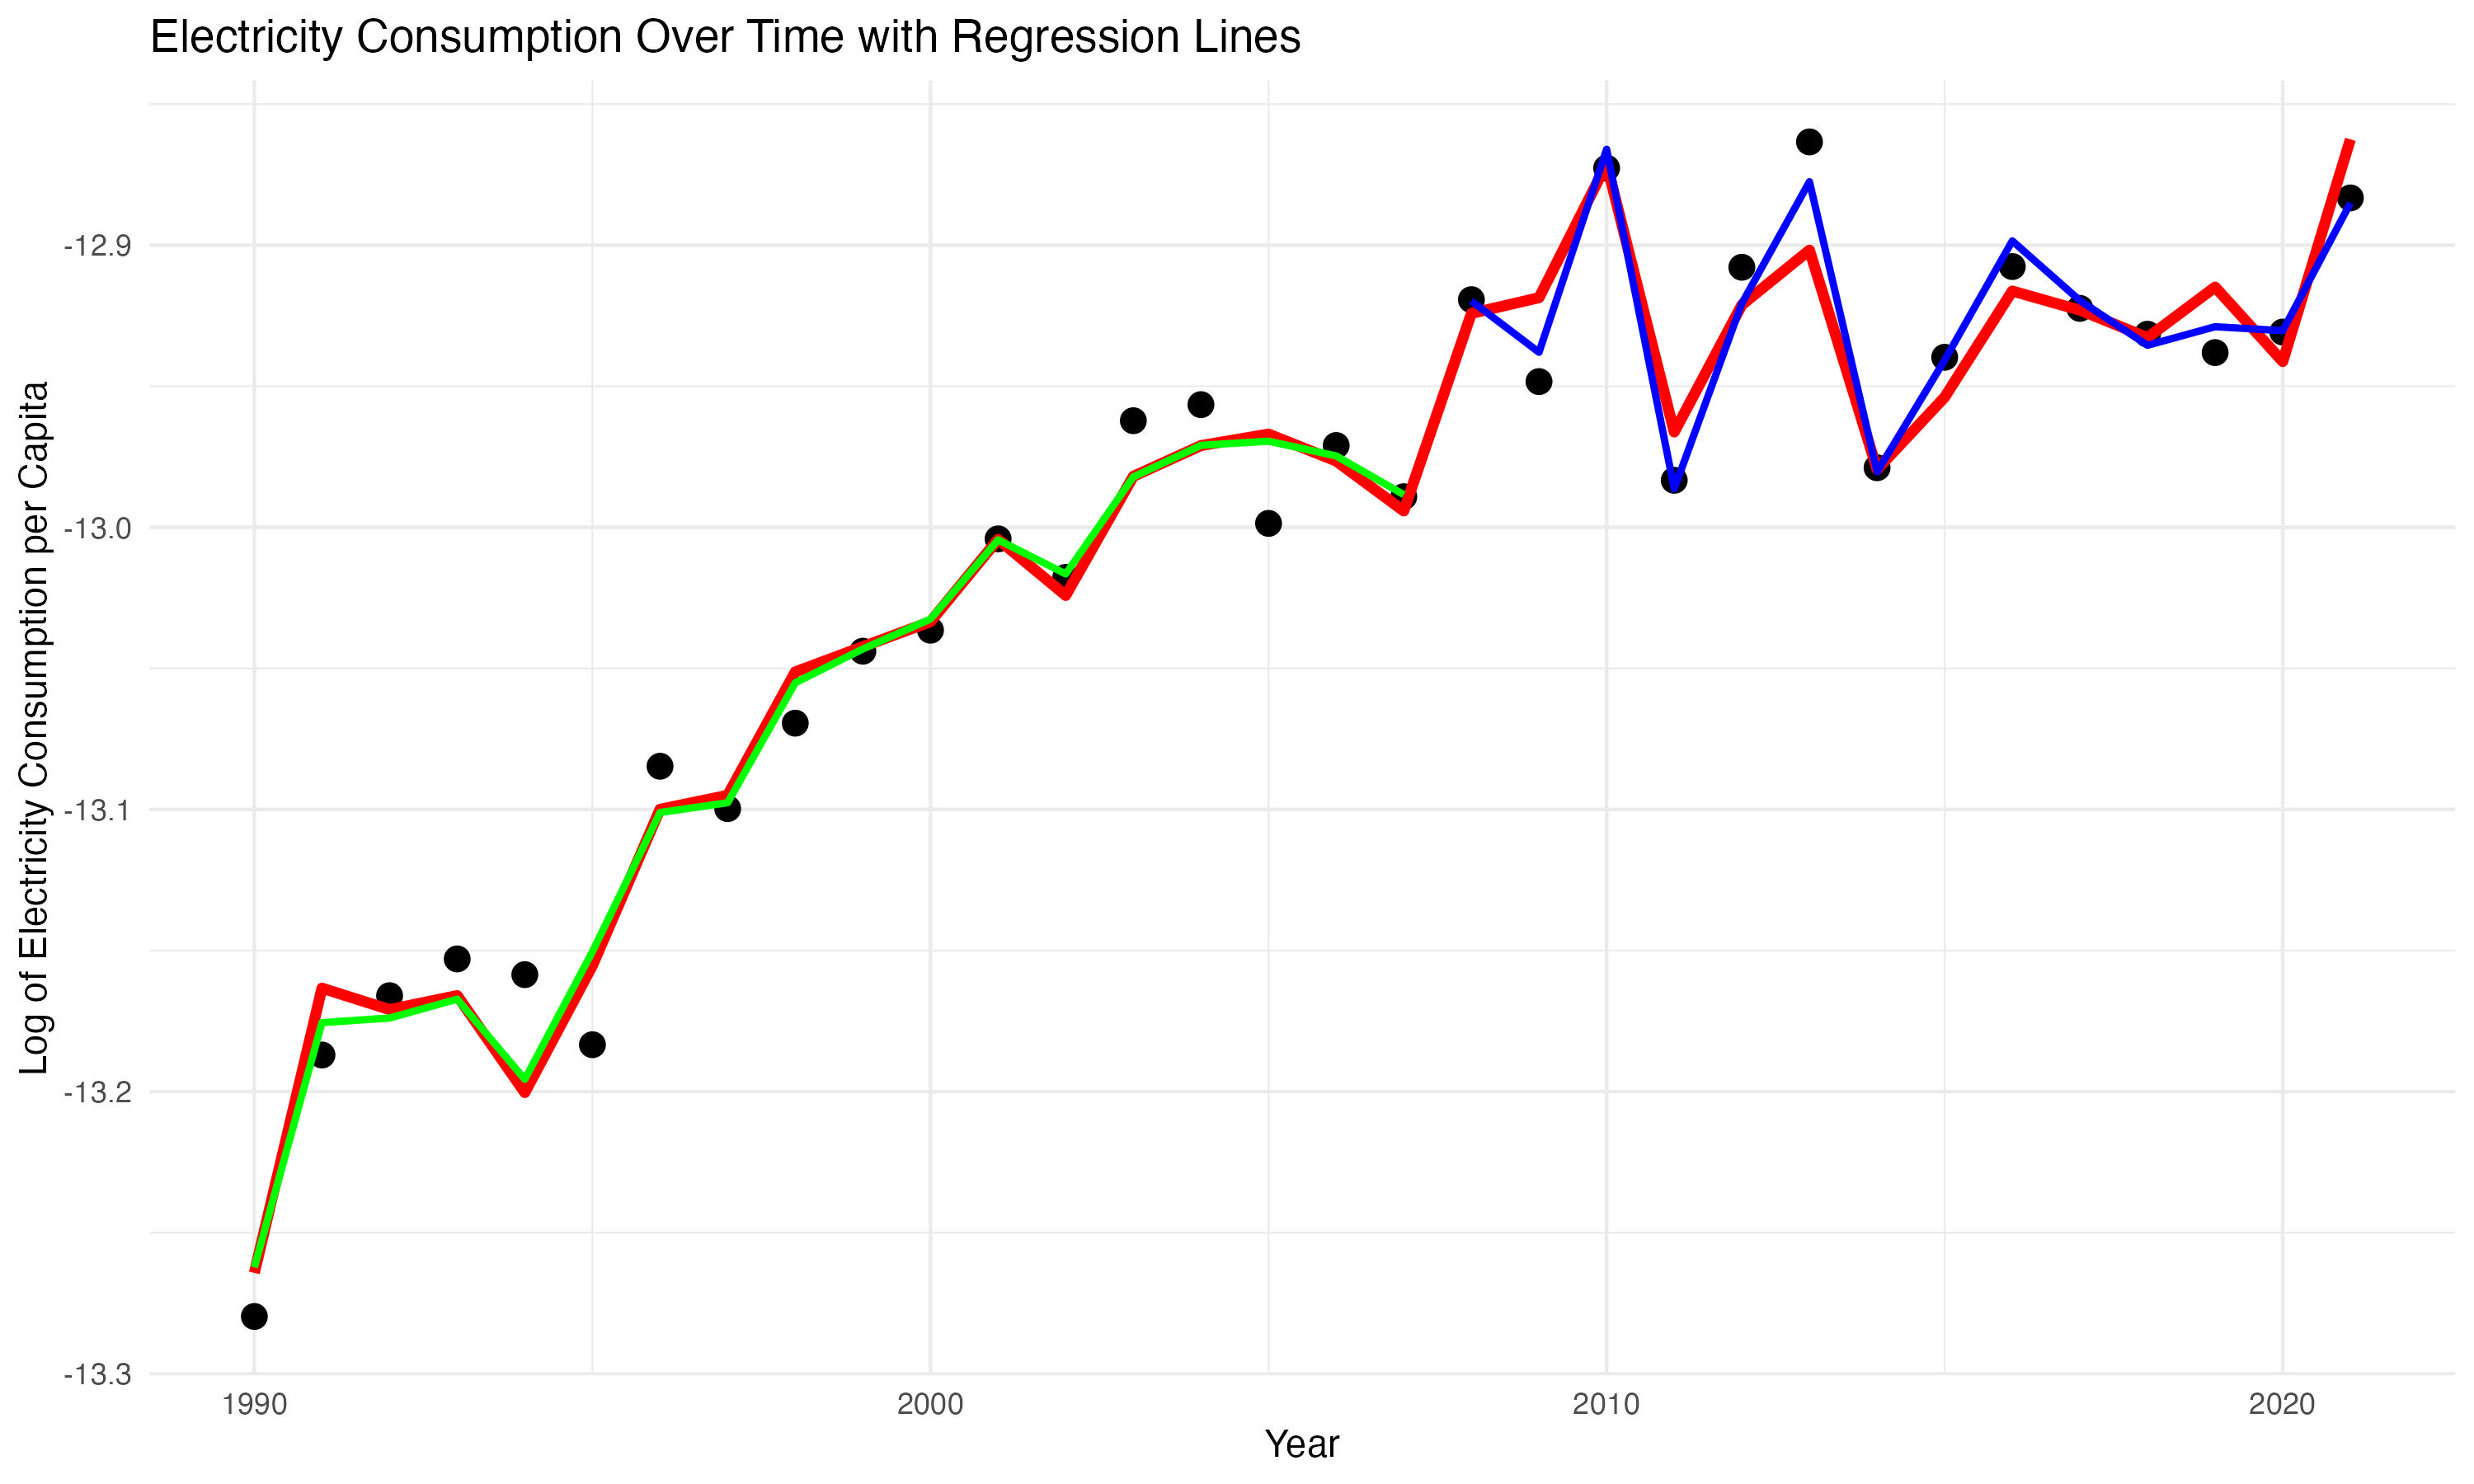
\includegraphics[width=0.5\textwidth]{Images/electricity_consumption_regression.jpeg}
      \caption{Observed and predicted logarithm of electricity consumption per capita. In green and blue are the predictions of the models \eqref{eq:before-after} (respectively before and after the break) and in red the predictions of the model \eqref{eq:break}.}
    \label{fig:regstructural}
  \end{figure}

\section{Forecasting to 2030}
Consistently with what we built, we will forecast the electricity consumption based on econometric relationships, especially on the model \eqref{eq:before-after}, considering values after 2007. Because we restrained ourselves with the methods taught in class, the electricity consumption forecast is based on very simple relationships and relies on the OLS coefficient estimated table \ref{regression_after}. Bootstrapping has been used in order to compensate for the low sample size. Nonetheless, it is clearly not enough to provide a satisfying forecast, as we can see figure \ref{fig:forecast}. Especially, the climate fluctuations are absolutely not captured by the linear model as they elicit explicit non-linearities.

\begin{figure}[h]
    \centering
      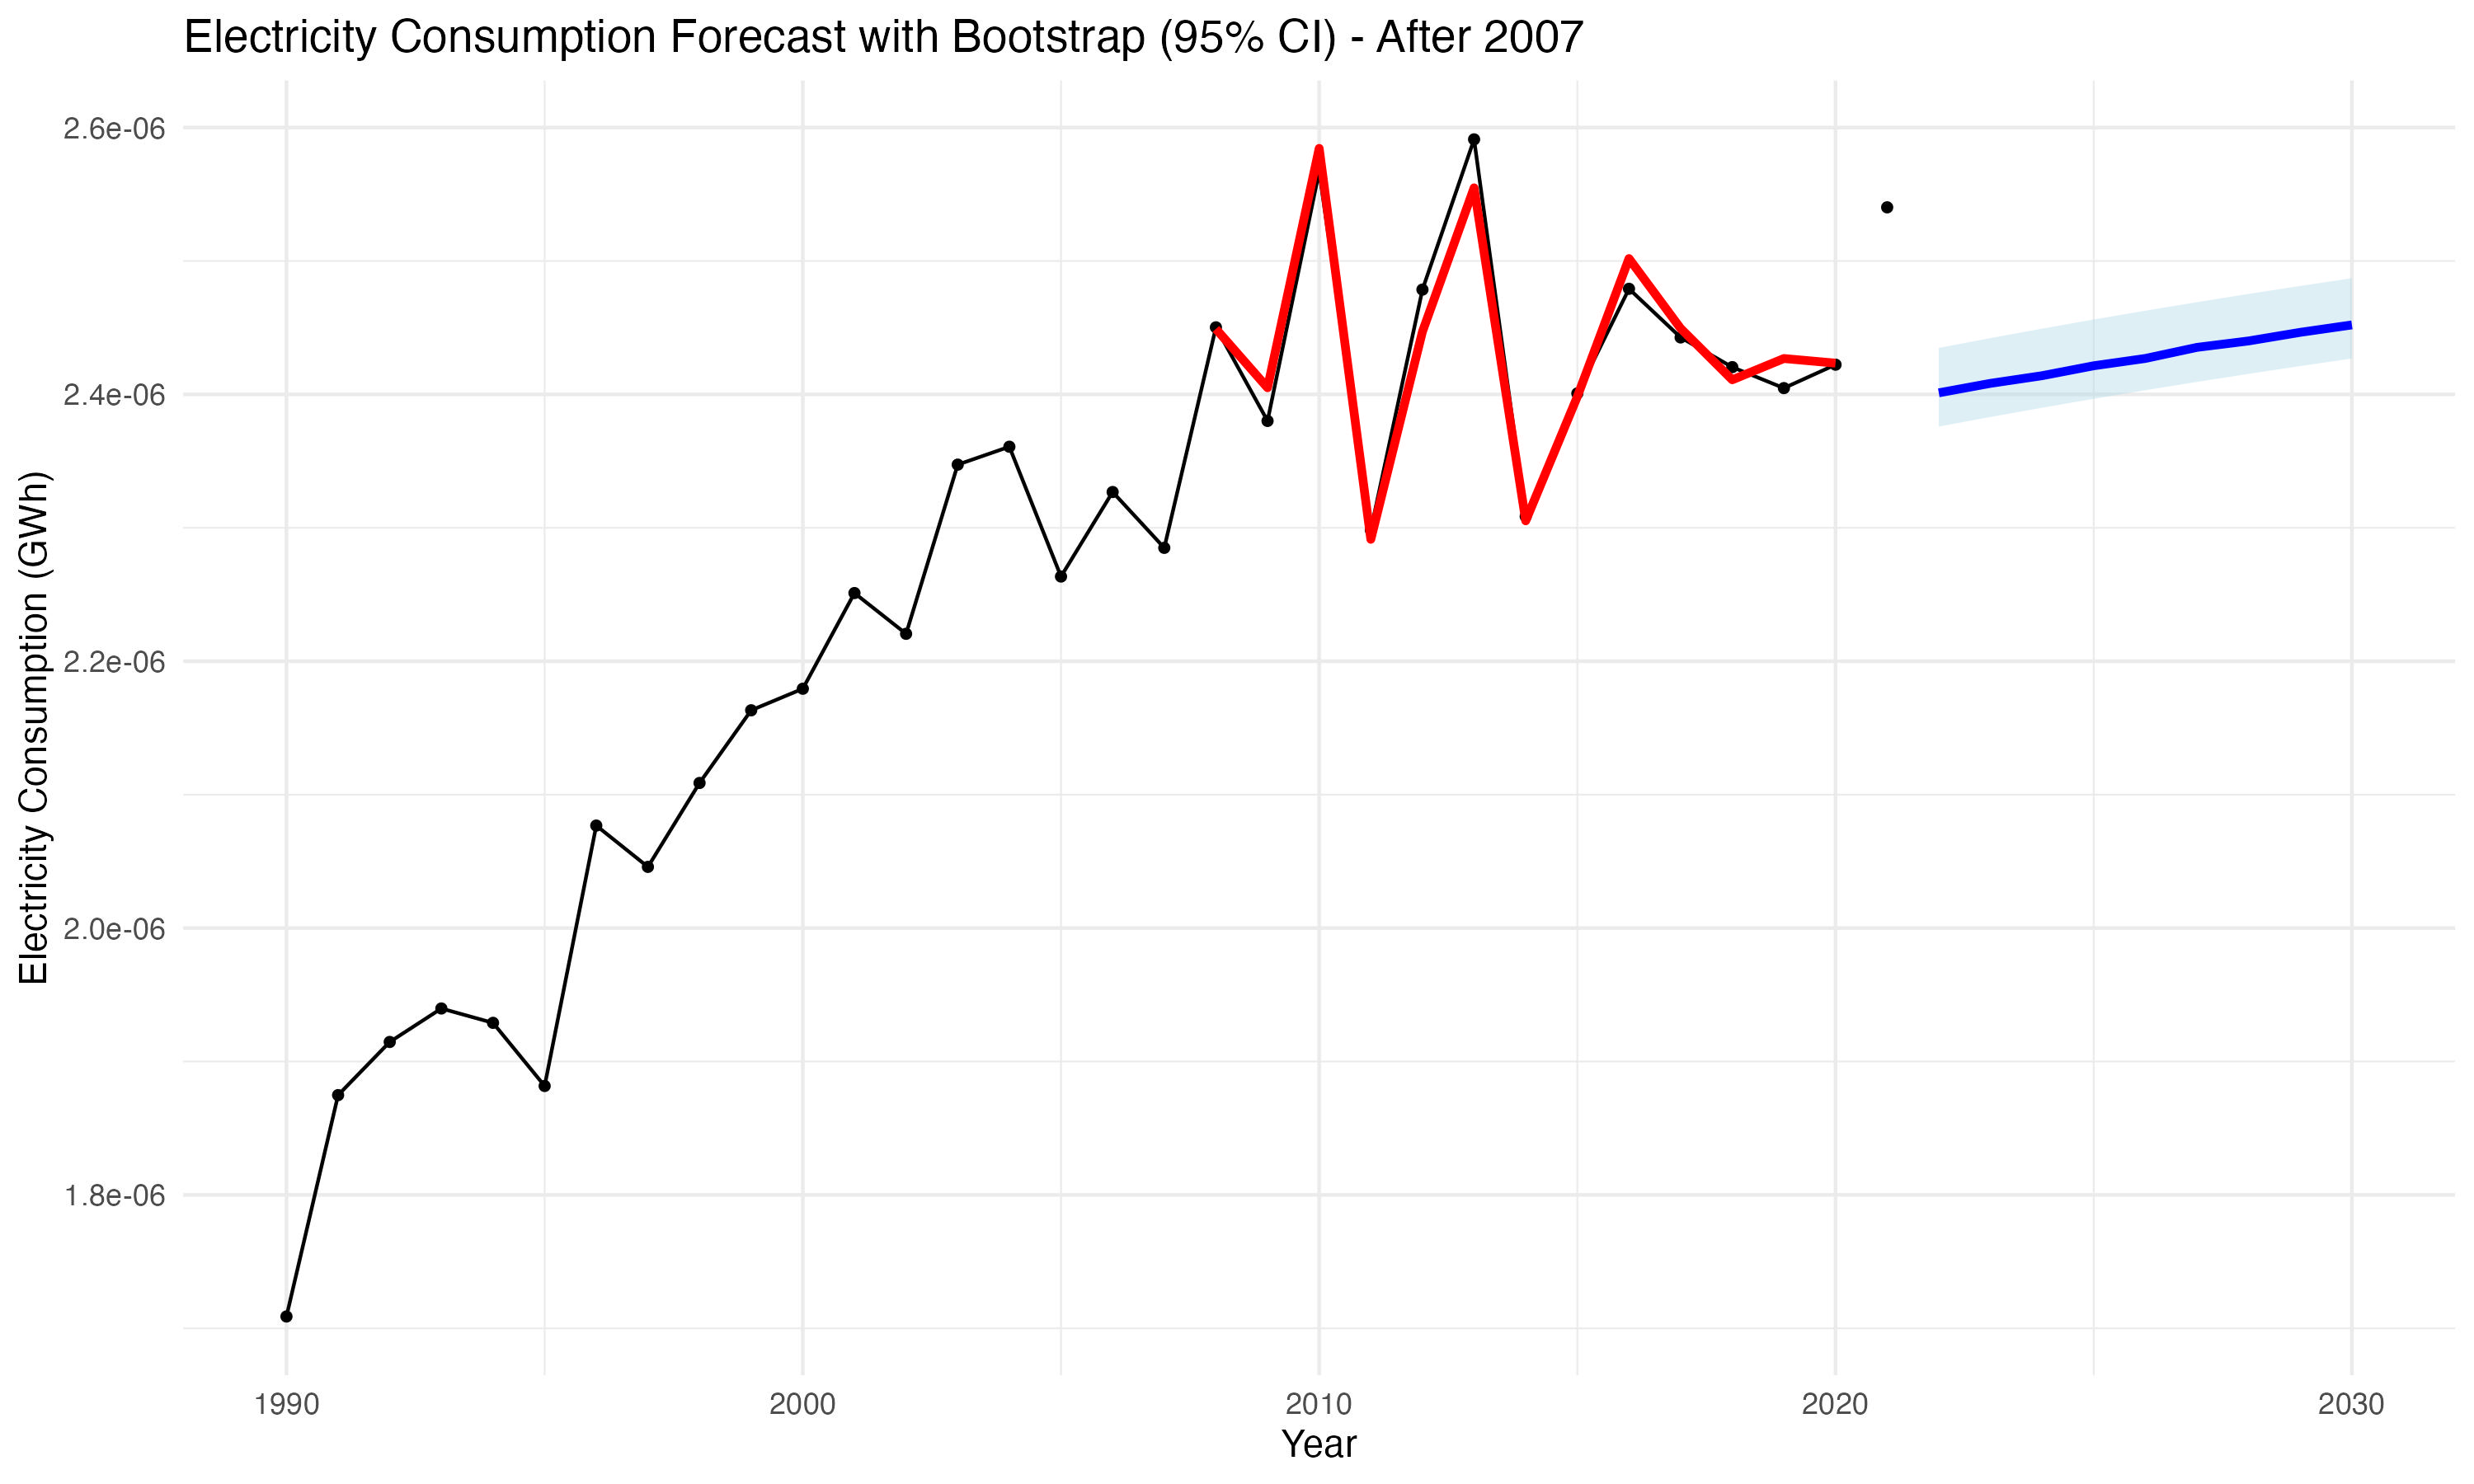
\includegraphics[width=0.5\textwidth]{Images/bootstrap_forecast_after.jpeg}
      \caption{Electricity consumption forecast from 2022 to 2030.}
    \label{fig:forecast}
  \end{figure}

\section{Discussion}
A more rigorous approach would have led us to at least use ARIMA models: we could have on one hand forecast the explanatory variables before using our model \eqref{eq:before-after} and on the other hand forecast the electricity consumption directly.

We would first have had to assess the weak exogeneity of the explanatory variables (the fact that their future values are not influenced by the dependent variable), which seems obvious for income, population, climate variations or inflation, that are not caused by eletricity consumption. For electricity price, we could have argued that electricity demand affects short-term pricing, but that long-term electricity price trends are mainly set by regulatory decisions and market forces. A Granger-Causality test actually confirms these assumptions. After checking stationarity of our univariate time-series (with a preference for the Elliott-Rothenberg-Stock (ERS), as it performs better for small samples), we would have find the integration order, the autoregressive order and the moving average order of the ARIMA model (with partial autocorrelation and autocorrelation functions). We could have defined a "seasonal" ARIMA model (SARIMA) for the climate index if needed. 

Nonetheless, all of this would have led to interpretation issues: why would we introduce lagged effect: do consumers take time to adjust to price changes? Does past prices or past income affect current consumption? About autoregression, does previous consumption influence current consumption? Our goal indeed was not to overfit the data to be as precise as possible but rather to elicit key microeconomic relationships that could explain the electricity consumption. The price effect and the income effect are well captured by the model, and the structural break is nicely detected as well.

Because no clear pattern was found, the use of a Markov-Switching process would not have been relevant. However, some non-linear terms could probably have been introduced in the model, especially to capture the effect of climate fluctuations. 

More interestingly, the use of a Vector Autoregression (VAR) model could have been welcomed to capture the interdependencies between the variables. It would have allowed us to forecast the electricity consumption and the electricity price simultaneously, taking into account the feedback effects between the two variables. Using a structural VAR would even have gave us the possibility to shock a variable (\textit{e.g.} as a simulation for a future crisis, or a policy implementation) and obtain an Impulse Response Function from the variables. We would however have need much more granular data, and a clear identification of the variables ordering to design the Cholesky decomposition.

Eventually, we mentioned the endogeneity issue: should the electricity price be considered as an endogenous variable from the moment energy markets were liberalized? When prices are no longer set by public authorities, their variation could indeed be explained by the demand for electricity: the use of instrumental variables would then have been necessary to avoid endogeneity bias. Dealing with COVID outliers also remains a challenge to be solved.

\newpage
